\documentclass[11pt,a4paper,svgnames]{article}
\usepackage{pgfgantt}
\usepackage{fancyhdr}
\usepackage{graphicx}
\usepackage{url}
\pagestyle{fancy}
\fancyhf{}% to clear existing header/footer if you don't want it
\renewcommand\headrulewidth{0pt}
\usepackage{xcolor}
\usepackage[scale=0.875]{geometry}
\usepackage{mathabx}
\usepackage{multicol}
\usepackage[alpine,weather]{ifsym}
\usepackage[skins]{tcolorbox}
\usepackage{academicons}
\usepackage{fontawesome}
\usepackage{tabularx}
\usepackage{booktabs}
\usepackage{hyperref}
%\usepackage{chronology}
\usepackage{chronosys}
\usepackage{tikz}
\usepackage{titlesec}

\newcommand*\circled[1]{\tikz[baseline=(char.base)]{\node[shape=circle,draw,inner sep=2pt] (char) {#1};}}

\newlength{\logowidth}
\setlength{\logowidth}{1.5cm} 
\setlength{\itemsep}{-.1cm}
\newcommand{\sepa}{$\cdot$~}
\usepackage{fontspec}
\setmainfont{Lato-Regular}

\definecolor{CVblue}{HTML}{1483D3}
\definecolor{CVorange}{HTML}{FFA034}
\definecolor{CVgrey}{HTML}{E3E3E3}
\definecolor{CVmain}{HTML}{3BA647}

\urlstyle{sf}
\DeclareUrlCommand\doi{\textcolor{CVmain}{\aiDoi}\def\UrlLeft##1\UrlRight{\nobreakspace\href{http://dx.doi.org/##1}{##1}}\urlstyle{sf}}

\DeclareGraphicsExtensions{.pdf,.png,.PNG,.JPG,.jpg,.jpeg,.gif}
\graphicspath{
{/home/ctroupin/Presentations/figures4presentations/logo/},
{./figures/}
}

\fancyfoot[R]{\begin{tcolorbox}[colback=CVgrey,colframe=CVmain,fonttitle=\bfseries,nobeforeafter,sidebyside,left=1mm,right=2mm,width=2.5cm,sidebyside align=top]
\thepage \end{tcolorbox}
}

\usepackage{array}
\newcolumntype{L}[1]{>{\raggedright\let\newline\\\arraybackslash\hspace{0pt}}m{#1}}
\newcolumntype{C}[1]{>{\centering\let\newline\\\arraybackslash\hspace{0pt}}m{#1}}
\newcolumntype{R}[1]{>{\raggedleft\let\newline\\\arraybackslash\hspace{0pt}}m{#1}}

\newtcbox{\skillbox}{nobeforeafter,colframe=CVmain,colback=CVgrey,boxrule=1pt,arc=4pt,height=0.5cm,
  boxsep=0pt,left=3pt,right=3pt,top=2.5pt,bottom=2pt,box align=center}
  
  \newtcolorbox{summarybox}[1][]{colback=white,
colframe=black,fonttitle=\bfseries,
colbacktitle=CVmain,enhanced,
attach boxed title to top center={yshift=-2mm},
title=Summary,#1}

% for the bibliography
% --------------------

\usepackage{multibib}
\newcites{article,incollection,conference}{{\faFilePdfO~Articles},{\faBook~Book chapters},{\faMicrophone~Talks and posters}}

\renewcommand{\labelitemi}{|} 

\hypersetup{
    urlcolor=CVblue,
    colorlinks=true,
    pdfauthor={Charles Troupin},
    pdftitle={Curriculum},
    pdfsubject={Never forget the metadata!},
	}

\titleformat{\section}{\normalfont\Large\bfseries}{\circled{\thesection}~--}{.4em}{}
\titleformat{\subsection}{\normalfont\bfseries}{\thesubsection~--}{.4em}{}

\begin{document}

\section{Contact data}

\begin{tabular}{L{.02\textwidth}L{.42\textwidth}L{.02\textwidth}L{.5\textwidth}}
\faEnvelopeSquare  	& charles.troupin@gmail.com 								& \faSkype			& charles.troupin1 \\
\faLinkedinSquare 	& \url{https://www.linkedin.com/in/charlestroupin/}		& \faGithubSquare	& \url{https://github.com/ctroupin/} \\
\aiOrcidSquare 		& \url{https://orcid.org/0000-0002-0265-1021} 	& \aiResearchGateSquare &\url{https://www.researchgate.net/profile/Charles_Troupin}\\
\faTwitterSquare	& \url{https://twitter.com/CharlesTroupin}		&  	& \\
\end{tabular}

\section{Experience}

%---------------------timeline----------------%
\begin{chronology}[align=left, startyear=2005,stopyear=2021, height=0pt, startdate=false, stopdate=false, dateselevation=0pt, arrow=false, box=true]
\chronograduation[event][dateselevation=0pt]{5}

\chronoperiode[textstyle=\raggedleft\colorbox{CVgrey},color=CVmain, startdate=false, bottomdepth=0pt, topheight=8pt, textdepth=-25pt,dateselevation=16pt,stopdate=false,datesseparation=/]{9/1/2017}{31/12/2020}{
\includegraphics[width=\logowidth]{logo_uliege}~
\includegraphics[width=.7\logowidth]{logo_gher}}

\chronoperiode[textstyle=\raggedleft\colorbox{CVgrey},color=CVblue, startdate=false, bottomdepth=0pt, topheight=8pt, textdepth=-25pt,dateselevation=16pt,stopdate=false,datesseparation=/]{14/3/2014}{8/1/2017}{
\includegraphics[width=\logowidth]{logo_socib}}

\chronoperiode[textstyle=\raggedleft\colorbox{CVgrey}, color=CVmain, startdate=false, bottomdepth=0pt, topheight=8pt, textdepth=-25pt,dateselevation=16pt,stopdate=false,datesseparation=/]{1/3/2013}{14/3/2014}{\includegraphics[width=.5\logowidth]{logo_imedea_s}}

\chronoperiode[textstyle=\raggedleft\colorbox{CVgrey}, color=CVblue, startdate=false, bottomdepth=0pt, topheight=8pt, textdepth=-25pt,dateselevation=16pt,stopdate=false,datesseparation=/]{1/10/2010}{28/2/2013}{
\includegraphics[width=\logowidth]{logo_uliege}}

\chronoperiode[textstyle=\raggedleft\colorbox{CVgrey}, color=CVmain, startdate=false, bottomdepth=0pt, topheight=8pt, textdepth=-25pt,dateselevation=16pt,stopdate=false,datesseparation=/]{1/10/2006}{30/9/2010}{\includegraphics[height=8mm]{FRS_FNRS_BLACK_transp.png}~\includegraphics[height=8mm]{logo_ulg.png}}

%\chronoperiode[textstyle=\raggedleft\colorbox{CVgrey}, color=CVorange, startdate=false, bottomdepth=0pt, topheight=8pt, textdepth=-25pt,dateselevation=16pt,stopdate=false,datesseparation=/]{1/9/2005}{30/9/2006}{\footnotesize{DEA in Oceanography}}

\end{chronology}

\begin{description}
\item[2017/01 present | Senior researcher |] GeoHydrodynamics and Environment Research (\href{http://modb.oce.ulg.ac.be/}{GHER})

\begin{itemize}%
\item Improvement and testing of the DIVA and DIVAnd interpolation software tools.
\item User support and training, documentation writing.
\item Analysis of suspended particular matter satellite images in the North Sea.
\item Interpolation of velocity measurements using HF radar and drifters.
\end{itemize}


\item[2014/03--2017/01 | Head of Data Centre |] Balearic Islands Coastal Ocean Observing and Forecasting System (\href{http//www.socib.eu}{SOCIB})
\begin{itemize}%
\item Management of the projects and staff.
\item Relations with external users (national and European), data providers and other facilities.
\item Development of applications for the access and visualisation of oceanographic data.
\item Forecasting of extreme sea level events (\textit{rissaga}) using time series.
\item Acquisition and processing of satellite, remote-sensing data\\(wind, salinity sea surface temperature, chlorophyll concentration).
\item Analysis and interpretation of multi-platform observations\\(HF radar, satellite, stations, mobile platforms).
\end{itemize}


\item[2013/03--2014/03 | Post-doctoral researcher |] Mediterranean Institute for Advanced Studies (\href{http://imedea.uib-csic.es/}{IMEDEA})
\begin{itemize}%
\item Preparation of high-resolution altimetry products in the Mediterranean Sea (MyOcean~2 project).
\item Analysis of in situ and remote-sensed data in the Balearic Sea.
\item Processing (interpolation, filtering) and interpretation of multi-sensor measurements\\(High-frequency radar, underwater glider, altimeter).
\item Operational production of regional altimetry maps (satellite imagery).
\end{itemize}


\item[2010/10--2013/02 | Research assistant |] \href{www.ulg.ac.be}{University of Li\`{e}ge}
\begin{itemize}%
\item Supervisor of the laboratory "\textit{Microscopes}" for undergraduate students\\ (laboratory sessions for 60-80 students, evaluation).
\item Analysis of total-suspended matter images on the North Sea.
\item Spatio-temporal interpolation of satellite wind data.
\item Improvement and testing of DIVA interpolation software tool.
\end{itemize}


\item[2006/10--2010/09 | PhD Candidate |] Fund for Research Training in Industry and Agriculture (\href{https://www.fnrs.be}{National Fund for Scientific Research}, Belgium), GeoHydrodynamics and Environment Research (\href{http://modb.oce.ulg.ac.be/}{GHER}, University of Li\`{e}ge)

\parbox{.65\textwidth}{
\begin{itemize}%
\item Study of the upwelling filament off Cape Ghir (Northwest Africa).
\item Hydrographic climatology for the North-East Atlantic Ocean.
\item Implementation of the ROMS model at high-resolution around Cape Ghir and design of process-oriented experiments.
\item Participation to the CAIBEX cruise onboard \textit{Sarmiento de Gamboa} (summer 2009) off Cape Ghir and processing of the cruise data.
\end{itemize}
}\hspace{.5cm}\parbox{.25\textwidth}{
\skillbox{MATLAB} \skillbox{ROMS} \skillbox{DIVA} \skillbox{Spatial interpolation} \skillbox{Quality control}
}


\item[2010/08--2010/09 | Trainee |] NATO Undersea Research Center, La Spezia (Italy)

\parbox{.65\textwidth}{
\begin{itemize}%
\item Development of an operational, multivariate processing for the reconstruction of incomplete satellite images.
\item Pre-processing of remote-sensed data (chlorophyll concentration, sea surface temperature).
\end{itemize}
}\hspace{.5cm}\parbox{.25\textwidth}{
\skillbox{MATLAB}\skillbox{DINEOF}
\skillbox{Remote sensing}
\skillbox{Multivariate analysis}
\skillbox{EOF analysis}
}


\item[2005/10--2005/12 | Research Engineer |] University of Li\`{e}ge

\parbox{.65\textwidth}{
\begin{itemize}
\item Modeling of Coccolithophore blooms in the Bay of Biscay using a 1-dimensional model (GOTM)
\end{itemize}
}\hspace{.5cm}\parbox{.25\textwidth}{
\skillbox{Fortran}\skillbox{MATLAB}
\skillbox{netCDF}\skillbox{Atmospheric forcing}
}
\end{description}


\section{Main research interests}

\begin{itemize}
\item {Data visualisation in environmental sciences}
\item {Spatial interpolation techniques applied to geophysical data}
\item {Processing and analysis of satellite images}
\item {High-resolution numerical modelling in coastal areas}
\item {Air-sea interactions and influence of physical processes on biology}
\end{itemize}
%


%\newpage
%-------------------
\section{Education}
%-------------------

\begin{description}
\item[2006--2011 | PhD in Sciences -- Oceanography |] University of Li\`{e}ge and University of Las Palmas de Gran Canaria: \emph{Study of the Cape Ghir upwelling filament using variational data analysis and regional numerical model}\\
\faUser~Supervisors: J.-M.~Beckers and P.~Sangr\`{a}\\
\faCalendar~Lecture date: 15 September 2011\\
\href{http://hdl.handle.net/2268/105400}{\faLink~http://hdl.handle.net/2268/105400}

\item[2005--2006 | Advanced Master in Modelling of the Marine Environment |] University of Li\`{e}ge and University of Las Palmas de Gran Canaria\\
Final project: \emph{Simulation of annual cycles of phytoplankton, zooplankton and nutrients using a mixed layer model coupled with a biological model}\\
\faUser~Supervisor: P.~Sangr\`{a}\\
\href{http://hdl.handle.net/2268/112587}{\faLink~http://hdl.handle.net/2268/112587}

\item[2000--2005 | Civil Engineer in Physics | ] University of Li\`{e}ge\\
Final project: \emph{Structuring in granular media}\\
\faUser~Supervisors: P.C.~Dauby and N.~Vandewalle (ULg)\\
\href{http://hdl.handle.net/2268/112588}{\faLink~http://hdl.handle.net/2268/112588}


\end{description}


\subsection{Training}

\begin{description}
\item[2019/11/29]{\textit{Professional software dedicated to research}, ULiège (3h), J.~Fays, R.~Hoyoux}
\item[2019/11/29]{\textit{Software development strategy}, ULiège (3h), J.~Fays}
\item[2018/01/21]{\textit{Managing an international research team}, ULiège (3h), I.~Halleux}
\item[2016/07]{\href{https://www.futurelearn.com/courses/big-data-visualisation}{\textit{Big Data: Data Visualisation}}, 2~weeks / 2~hours per week, Queensland University of Technology}
\item[2016/06]{\href{https://www.codecademy.com/learn/sql-table-transformation}{\textit{SQL: Table Transformation}}, Code Academy}
\item[2016/06]{\href{https://www.codecademy.com/learn/learn-sql}{\textit{Learn SQL}}, Code Academy}
\item[2016/01]{\href{https://www.meted.ucar.edu/training_module.php?id=993}{\textit{Tropical Mesoscale Convective Systems}}, 1.5 hour, Comet MedEd}
\item[2016/01]{\href{https://www.meted.ucar.edu/training_module.php?id=1093}{\textit{Using Scatterometer Wind and Altimeter Wave Estimates in Marine Forecasting}}, 2 hours, Comet MedEd}
\item[2015/12]{\href{https://www.futurelearn.com/courses/climate-from-space}{\textit{Monitoring Climate from Space}}, 5~weeks / 3~hours per week, European Space Agency}
\item[December 2015]{\href{https://developers.google.com/edu/python/?hl=en}{\textit{Google's Python Class}}, 2 days, Google for Education}
\item[2012/11/06]{\textit{Interview in English}, Gembloux (1~day), J.-P. Hermann}
\item[2012/10/26]{\textit{Understanding the factors of success and failure in the first year of university}, ULg (1/2~day), L.~Leduc and B.~M\'{e}renne}
\item[2012/10/24]{\textit{Keys and main principles of team management}, ULg  (1/2 day), L. Mar\'{e}chal}
\item[2012/05/10]{\textit{Efficient slides and graphics}, ULg (2h), J.-L. Doumont (Principi\ae)}

\item[2011]{\textit{Structuring written documents}, ULg (2h), J.-L. Doumont (Principi\ae)}
\end{description}


\newpage

%--------------------------------------
\section{Skills and Competencies}
%--------------------------------------

\subsection{Technical skills}

\begin{description}

\item[Data analytics] Quality control, Time series analysis, Singular events, Filtering, Data mining, Statistics, Predictive modelling

\item[Engineering] Fluid mechanics, Aerodynamics, Finite-Element Method, Atmospheric Physics, Numerical simulations, Numerical analysis, Signal processing, Optimization, High-performance computing

\item[Physical Oceanography] Spatial interpolation, Time-Series Analysis, Principal Component Analysis, Process-oriented modelling, Database Management, Satellite Image Processing

\end{description}


\subsection{IT skills}

\subsubsection*{\circled{\faCode}~~Programming}
Functional programming 				\\ 
Object oriented programming		\\
Test-oriented development			\\
Control version system (git, svn)	\\
Unit testing						\\	
Continuous integration

\subsubsection*{Languages}
\ganttset{bar height=.3}
\begin{ganttchart}[
	canvas/.style={fill=white},
    hgrid style/.style={draw=black!5, line width=.75pt},
    vgrid={*1{draw=CVmain, line width=.75pt, dashed},*2{draw=CVgrey, line width=.75pt, dashed}},
    title/.style={draw=none, fill=none},
    title label font=\bfseries,
    title label node/.append style={below=7pt},
    include title in canvas=false,
    bar label font=\mdseries\small\color{black!70},
    bar label node/.append style={left=.2cm},
    bar/.append style={draw=none, fill=black!63},
    bar incomplete/.append style={fill=black!70},
    bar progress label font=\mdseries\footnotesize\color{black!70},
    bar progress label node /.style=east,
    y unit chart=.5cm,
    progress=today,
    today=1,
    today label={}, 
    today rule /.style={draw=CVmain, line width=.75pt, dashed},
    progress label text = ,
    ]{1}{17}
  % \gantttitle[title label node/.append style={below left=5pt and -3pt}]{Languages\quad}{0}
  %\gantttitle[title/.style={draw=CVmain,below=7pt}]{Languages}{0}
  \gantttitlelist[title/.style={draw=none, inner color=CVgrey,below=7pt}]{2006,2009,...,2020}{3} \\
  \ganttbar[name=bash, progress label text={awk, makefiles, cron, ssh, regex, \ldots}]{Bash}{1}{16} \\
  \ganttbar[name=fortran,progress label text={\hspace{.5cm}data I/O, format conversion, optimisation}]{Fortran}{1}{15} \\
  \ganttbar[name=matlab,progress label text={\hspace{4cm}geostatistics, plotting, neural networks, m\_map}]{MATLAB}{1}{8} \\
  \ganttbar[name=python,progress label text={matplotlib, numpy, scipy, pandas, virtualenv, Basemap, \ldots}]{Python}{8}{16} \\
  \ganttbar[name=julia,progress label text={DataArrays, PyPlot, module developments}]{Julia}{11}{16} \\
  \ganttbar[name=javascript,progress label text={Leaflet, Highcharts, D3, Angular, Reveal}]{Javascript}{11}{16}\\
  \ganttbar[name=Tcl/Tk,progress label text={\hspace{7cm}Graphical interface (buttons, file selectors, \ldots)}]{Tcl/Tk}{1}{2}\\
  \ganttbar[name=LaTeX,progress label text={Beamer, TikZ, BibTeX, tcolorbox, \ldots}]{LaTeX}{1}{16}
\end{ganttchart}

\subsubsection*{\circled{\faWrench}~~Tools}

\begin{description}
\item[Visualisation:] bokeh, matplotlib, folium, plotly, leaflet, cartopy
\item[Data bases:] MySQL, PostgreSQL
\item[Operating systems:] Linux (Mint, Ubuntu) \sepa Experience with Mac~OS~X Lion, Microsoft Windows
\item[Image processing:] GIMP, Inkskape, Darktable, ImageJ, Matlab, Python, ffmpeg, hugin, ImageMagick
\item[Oceanography software:] Ocean Data View, DIVA (spatial interpolation), DINEOF (spatio-temporal interpolation of satellite images)
\item[Misc:] NX~Client, VPN, Asana, QGIS
\end{description}


\subsection{Management}

\begin{description}
\item[Projects and management] {Planning and monitoring, scientific and technical reports, teamwork, deadlines, specification documents, applications for grants and supports.}

\item[Communication] {Oral presentations at international conferences (in English, Spanish or French), social networking, management of group accounts on twitter (\symbol{64}SOCIB\_data, \symbol{64}GHER\_ULg).}

\item[Conference organisation]{Main organiser of several editions of the Diva workshop (10 participants from European research centres on average) and member of the organising committee of the 48th International Li\`{e}ge Colloquium on Ocean Dynamics (200 participants from 40 countries).}

\end{description}


\subsection{Languages}
\begin{summarybox}
English for the communication with the project partners and for the writing of technical document. Spanish, English and Catalan in the previous working environment.
\end{summarybox}

\begin{description}
\item[French] {Native speaker}
\item[Spanish] {Highly proficient in spoken and written Spanish}
\item[English] {Highly proficient in spoken and written English}
\item[Catalan] {Limited working proficiency}
\item[German] {Limited working proficiency}
\item[Italian] {Elementary proficiency}
\item[Dutch] {Elementary proficiency (basic course for beginners)}
\end{description}

\subsection{Teaching and Training}

\begin{summarybox}
My experience of training at the University is complemented by several training courses given in the frame of European projects or invited lectures.
\end{summarybox}

\begin{description}

\item[2019/10/28--30] \textit{Introduction to scientific Python. Application to Oceanography}, University of C\'{a}diz, Facultad de Ciencias del Mar y Ambientales: Graduate students, researchers and professors.

\item[2017/11/15--17] \textit{Open Sea Lab Workshop}, De Serre, Antwerp: Participant coaching for the EMODnet data access and usage.

\item[2017/04] \textit{Geophysical Fluid Dynamics}, University of Li\`{e}ge, Facult\'{e} des Sciences: Master students.

\item[2016/01/27--29] \textit{Introduction to scientific Python. Application to Oceanography}, University of C\'{a}diz, Facultad de Ciencias del Mar y Ambientales: Graduate students, researchers and professors.

\item[2015/12/10--11] CMEMS Regional User Training Workshop dedicated to the Atlantic European South West Shelf Ocean, Lisbon (Portugal): data and tools of the In Situ Thematic Assembly Center (INSTAC). 
\item[2015/12/03--04] CMEMS Regional User and Training Workshop dedicated to the Mediterranean Sea, La Spezia (Italy): data and tools of the In Situ Thematic Assembly Center
\begin{itemize}
\item Manipulation of netCDF files.
\item Discovery and access to data.
\item Use of Python and Ocean Data View to process oceanographic data.
\end{itemize}
\item[2010/10--2013/02] \textit{Physics laboratory (optics)}, University of Li\`{e}ge, Faculty of Medicine and Faculty of Veterinary Medicine: Undergraduate students.
\item[2007--2013] \textit{Physical Oceanography, Risk Management, Marine Meteorology} (assistant), University of Li\`{e}ge, Faculty of Sciences: Undergraduate students.

\end{description}


%----------------------------------
\section{Projects and services}
%----------------------------------

\begin{summarybox}
{Since 2006, I have been involved in several internal, national and European projects dealing with data analysis and management, operational oceanography or numerical modelling. I contributed to the project proposals, the preparation of the deliverables, the support to users and was participating to the meetings of the technical task group and steering committee.}
\end{summarybox}

\subsection{European projects}

\begin{description}

\item[2019--ongoing] \href{https://www.phidias-hpc.eu/}{PHIDIAS} (CEF Telecom): Deployment of DIVAnd tool in a HPC environment.

\item[2019--ongoing] \href{https://www.emodnet-physics.eu}{EMODnet Physics}: Creation of velocity maps by interpolating drifter and high-frequency radar measurements.

\item[2018--ongoing] \href{https://www.eosc-hub.eu}{EOSC-Hub}: Development of a data analytics platform for marine data.

\item[2017--ongoing] \href{https://emodnet-biology.eu}{EMODnet Biology}: Creation of gridded fields based on species counts and observations.

\item[2017--ongoing] \href{https://www.emodnet-chemistry.eu}{EMODnet Chemistry} 
\begin{itemize}
\item Creation of gridded field for chemical variables.
\item Visualisation of the products using the OceanBrowser tool.
\item Preparation of merged products combining all the regional components.
\item Generation of XML records for the data catalog.
\end{itemize}

\item[2017--ongoing] \href{https://www.emodnet-ingestion.eu}{EMODnet Data Ingestion}: Development on new gridded products using the data obtained in the frame of the project.

\item[2017--ongoing] \href{https://www.seadatanet.org}{SeaDataCloud} (H2020): Further developing the pan-European infrastructure for marine and ocean data management
\begin{itemize}
\item Improvement and testing of the DIVA software tool.
\item Development of a user interface for Diva on a Virtual Research Environment.
\item Preparation of the new regional products.
\end{itemize}


\item[2015--2017] \href{http://www.jerico-ri.eu/}{JERICO-NEXT} (H2020): Data management best practices; glider data processing and calibration.
\item[2015--2017] \href{http://www.odip.eu/}{ODIP~2} (Ocean Data Interoperability portal)
\begin{itemize}
\item Test of new standards in data and metadata management 
\item Data visualisation tools
\end{itemize}

\item[2015--2017] Copernicus Marine Environment Monitoring Service, In Situ Thematic Assembly Center (INSTAC):
\begin{itemize}
\item Elaboration of the Ocean State Report.
\item Coordinator of the outreach, training and communication activities.
\item Preparation and participation to the regional user training workshops.
\end{itemize}

\item[2013--2014] MyOcean~2, Ocean monitoring and forecasting infrastructure:
\begin{itemize}
\item Preparation of high-resolution altimetry products in the Mediterranean Sea.
\item Data analysis during a multi-platform experiment in the Ibiza Channel.
\end{itemize}

\item[2012--2013] \href{http://www.odip.eu/}{ODIP} (Ocean Data Interoperability portal): Definition of standards for the data and metadata exchange.

\item[2011--2015] PERSEUS (Policy-oriented marine Environmental Research for the Southern European Seas): Processing of glider and campaign data

\item[2009--2013] \href{https://www.emodnet-chemistry.eu}{EMODnet -- Chemistry}: Pilot component for a final operational European Marine Observation and Data Network:
\begin{itemize}
\item Improvement to the DIVA tool.
\item Development of the DIVA web-interface.
\end{itemize}

\item[2009--2013] \href{https://www.seadatanet.org}{SeaDataNet~2}: Infrastructure for ocean and marine data exchange.

\item[2008--2009] CAIBEX (Study of the Exchanges between continental shelf and ocean in the Canaries-Iberian marine ecosystem):
\begin{itemize}
\item Implementation of a high-resolution numerical model in the Cape Ghir region.
\item Participation to the CAIBEX-Cape Ghir cruise (August 2009).
\end{itemize}

\item[2006--2011] \href{https://www.seadatanet.org}{SeaDataNet}: Infrastructure for ocean and marine data exchange:
\begin{itemize}
\item Contribution to the project proposal.
\item Development, documentation and testing of DIVA software tool.
\item Organization of the user training workshops.
\end{itemize}

\end{description}


\subsection{National projects}

\begin{description}
\item[2019--ongoing] Multisync: combination of satellites measurements at different resolutions to reconstruct suspended particular matter in the North Sea.
\item[2014--2017] BlueFin Tuna: combination of observations and models to understand and predict tuna abundance.
\item[2014--2017] Grumers: Database for jellyfish observations around the Balearic Islands. 
\item[2014--2017] \href{http://medclic.es/es/news/research/asimilacion-datos.html}{Medclic} (Oceanographic data in the Medirranean Sea at one click): Providing access to SOCIB sensors data.
\item[2014--2015] SeaTurtle: Development of a viewer showing turtle trajectories in real-time.
\item[2011--2013] HiSea (High-resolution merged satellite Sea surface temperature fields): EOF analysis of satellite images improved with numerical model outputs.
\item[2010/08] REP10 (Recognized Environmental Picture): Analysis and reconstruction of incomplete satellite images on the Ligurian Sea.
\end{description}

%----------------------------------
\section{Research stays}
%----------------------------------

\begin{description}
\item[3 September - 31 October 2018] Analysis of surface currents in the Gulf of Trieste using high-frequency radar, Marine Biology Station Piran, National Institute of Biology (NIB), Piran (Slovenia).
\item[5 August - 5 September 2010] Analysis of satellite images in the Ligurian Sea, NATO Undersea Research Centre (NURC), La Spezia (Italy). 
\item[15 July 2009 - 30 September 2009] Preparation and participation to CAIBEX cruise, Las Palmas (Spain) and Cape Ghir (Morocco). 
\item[5 January 2009 - 31 March 2009] Diagnostics on model outputs, ULPGC, Las Palmas de Gran Canaria (Spain).
\item[30 May - 30 August 2008] High-resolution configuration for the model, ULPGC.
\item[5 December 2007 - 5 March 2008] Diagnostics on model outputs, ULPGC.
\item[21 May - 24 August 2007] Design of process-oriented numerical experiments, ULPGC.
\item[5 January - 15 March 2007] Implementation of ROMS numerical model, ULPGC.
\end{description}



\section{Scientific contributions}
%%---------------------------------

\begin{summarybox}
In the frame of international projects, I authored or co-authored several works published in peer-reviewed journal and mainly focused on data analysis and tools.
\end{summarybox}

\begin{table}[h]
\centering
\begin{tabular}{C{4cm}C{4cm}C{4cm}}
\huge{20+}  	& \huge{100 +} & 	Reviewer for\hspace{1cm}  \\
Papers in peer-review journals & Presentations at international conferences	& \huge{7} \hspace{2cm} \normalsize{journals} \\
\end{tabular}
\end{table}

%\newpage


\nocitearticle{*}
\bibliographystylearticle{referencelist}
\bibliographyarticle{Troupin_publi.bib}

\nociteincollection{*}
\bibliographystyleincollection{referencelist}
\bibliographyincollection{Troupin_book.bib}
 
\nociteconference{*}
\bibliographystyleconference{referencelist}
\bibliographyconference{Troupin_conferences.bib}

\begin{center}
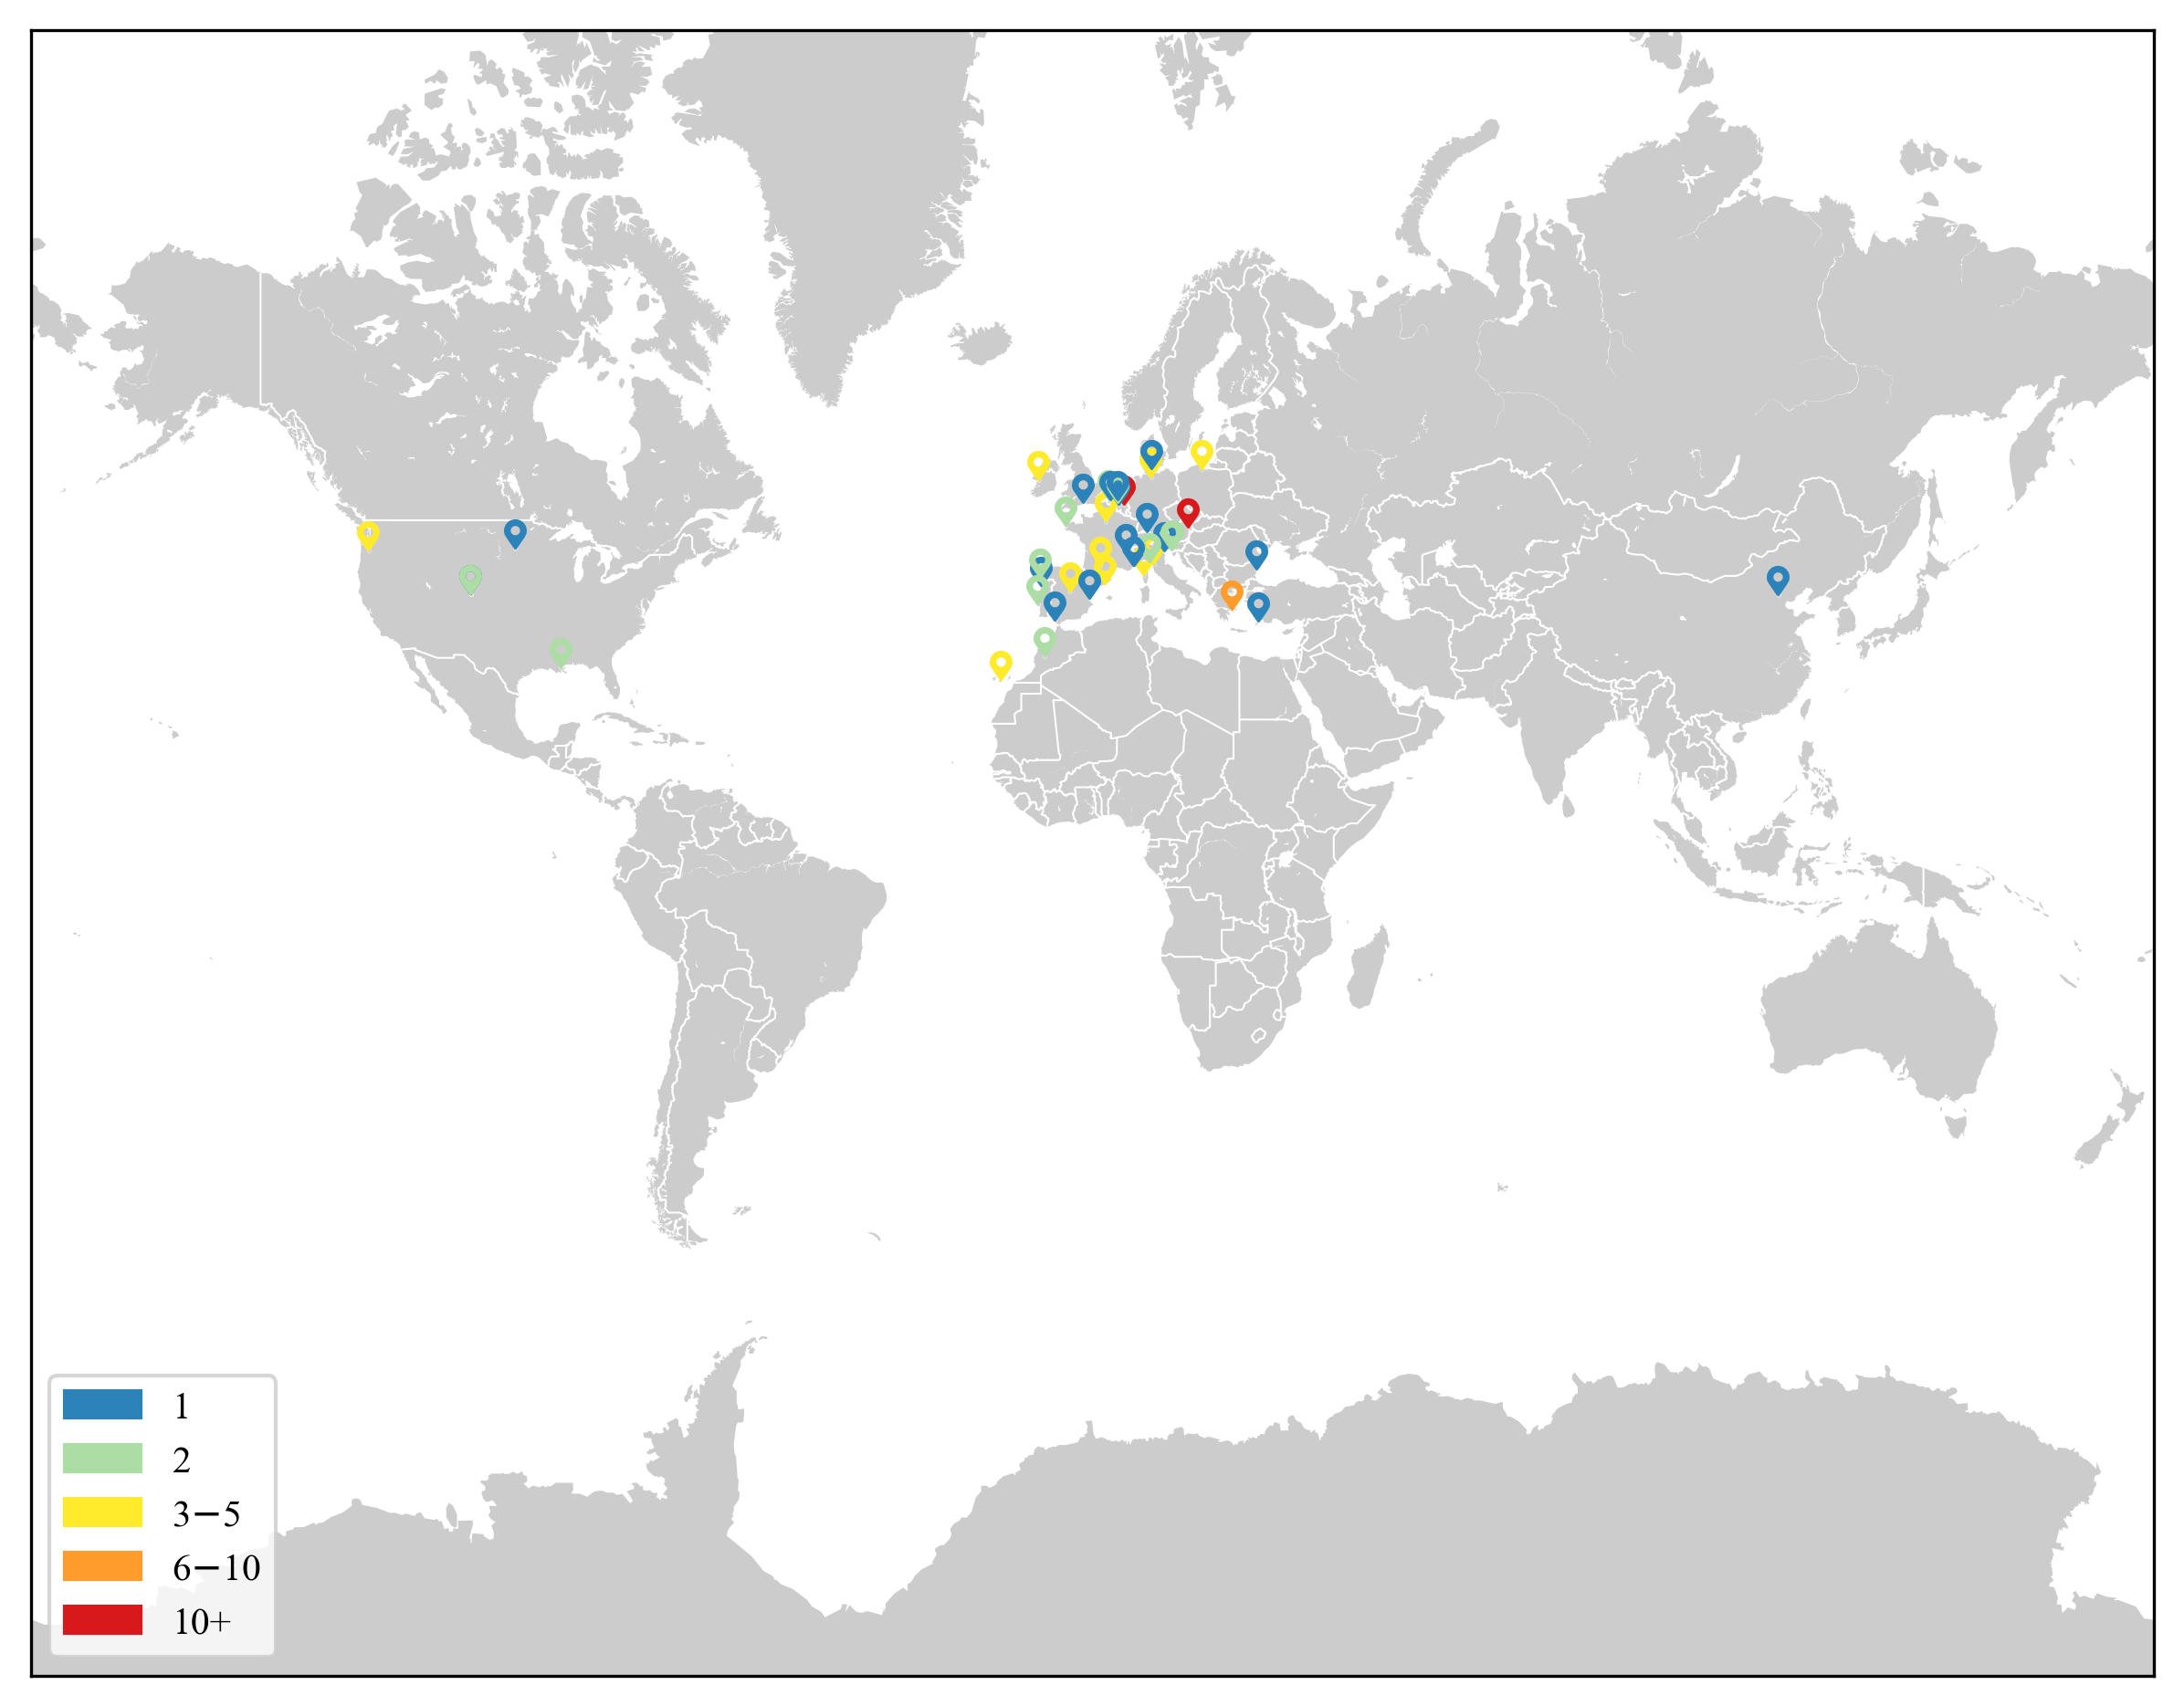
\includegraphics[width=.75\textwidth]{ConferenceMap.png}
\end{center}

\subsection{Invited Editor}

Ocean Dynamics: Special Issue for the 48th Li\`{e}ge Colloquium on Ocean Dynamics, \doi{10.1007/s10236-018-1173-5}

\subsection{Reviewer}

Earth System Science Data, Ocean Science, Ocean Dynamics, Ocean Engineering, Journal of Marine Systems, Journal of Geophysical Research -- Ocean, Remote Sensing of Environment

\subsection{Doctoral thesis tribunal}

\begin{description}
\item[2017/09/25] Bàrbara Barceló-Llull (ULPGC, Spain) {\newline \textit{Shedding light into mesoscale dynamics and vertical motion through synthetic and in situ observations}}

\item[2017/09/16] Yeray Santana Falc\'{o}n (ULPGC, Spain) {\newline \textit{Transport, Respiration, and Sequestration of Organic Carbon in the Canary Current Ecosystem: Relevance within the Global Carbon Cycle}}
\end{description}

\subsection{Undergraduate student training}
\begin{description}
\item[2012/05/12--2012/05/19] Joaquim Pereira Bento (Uni-Kiel, Germany)\\ \textit{In situ and satellite data interpolation}
\item[2011/09--2011/11] Nikolaos Zarokanellos (HCMR, Greece) \\ \textit{Data interpolation for the Eastern Mediterranean Sea}
\item[2009/01--2009/05] Marc Piedeleu (ULPGC, Spain)\\ \textit{Analysis of in situ observations south of the Canary Islands}
\item[2008/11--2008/12] Anna Rabitti (OGS, Italy)\\ \textit{Spatial interpolation of in situ data in the Adriatic Sea}
\end{description}

\subsection{Organisation of conferences}

\begin{summarybox}
From 2006 on, I have organised several editions of a training workshop about an interpolation software tool (DIVA) and helped in the organisation or the International Li\`{e}ge Colloquium on Ocean Dynamics. In 2016, I co-organised the 48th Edition on \textit{Submesoscale processes}, which gathered over 200 scientists from 40 countries.
\end{summarybox}

\begin{description}
\item[2016/05/23--27] 48th International Li\`{e}ge Colloquium on Ocean Dynamics on \textit{Submesoscale Processes: Mechanisms, Implications and new Frontiers} (Li\`{e}ge, Belgium)
\begin{itemize}
\item Invitation of keynote speakers.
\item Applications for sponsorship.
\item Preparation of the scientific program.
\item Design of the conference flyer.
\item Organisation of social events.
\end{itemize}

\item[2012/10/08--12] 6th Diva workshop (Roumaillac, France)
\begin{itemize}
\item Scientific content.
\item Invitation of the participants.
\item Logistic: meeting venue, transportation from/to the airport.
\end{itemize}

\item[2010/11/03--06] 5th Diva workshop (Calvi (France)
\item[2009/10/23--26] 4th Diva workshop (Calvi, France)
\item[2008/10/15--17] 3rd Diva workshop (Calvi, France)
\item[2007/11/04--06] 2nd Diva workshop (Calvi, France)
%\item[2012/05/07--11] 44th International Li\`{e}ge Colloquium on Ocean Dynamics on \textit{Remote sensing of colour, temperature and salinity -- new challenges and opportunities}}{Li\`{e}ge (Belgium)}
%\item[2010/04/26--30] {42nd International Li\`{e}ge Colloquium on Ocean Dynamic}{"\textit{Multiparametric observation and analysis of the Sea}"}{Li\`{e}ge (Belgium)}
\item[2006/11/13--15] 1st Diva workshop (Li\`{e}ge, Belgium)
\begin{itemize}
\item Workshop program.
\item General logistics. 
\end{itemize}
\end{description}

\section{Misc}

\subsection{Grants and funding}

\begin{description}
\item[2011/04 \& 2015/04] EGU Young Scientist's Travel Award
\item[2008/05--2008/09] Travel grant (French Community of Belgium)
\item[2006/10--2010/09] Fund for Research Training in Industry and Agriculture (National Fund for Scientific Research, Belgium)
\item[2006/02--2006/09] \textit{Erasmus} travel grant (European Commission)
\item[2005/09--2005/12] \textit{Pisart} supervision grant: creation of the presentation support for the course \textit{Thermodynamics of continuous media} in LaTeX% (Prof.~J.-P. Ponthot).}
\item[2004/02--2004/06] State grant: writing of the course notes for the course \textit{Further Study of Digital Analysis (Equations with Partial Derivatives)}% (Prof.~J.-A.~Essers).}
\end{description}

\subsection{Representation}
\begin{description}
\item[2017--ongoing] Delegate at the Department Council (Astrophysics, Geophysics and Oceanography, ULi\`{e}ge)
\item[2015--2016] Member of the Monitoring Committee of the Framework Agreement between AEMET and SOCIB
\item[2003--2005] Student delegate 
\item[2011--2013] Delegate at the Department Council (Astrophysics, Geophysics and Oceanography, ULi\`{e}ge)
\end{description}


\subsection{Memberships}

\begin{itemize}
\item European Geosciences Union (EGU)
\item American Geophysical Union (AGU)
\item Cloud Appreciation Society
\end{itemize}

\subsection{Personal interests}

\begin{itemize}
\item \href{http://www.wikiloc.com/wikiloc/user.do?id=458033}{Running}: trails, mountain races, track
\item \href{https://500px.com/charlestroupin}{\faicon{500px}}~\href{https://www.flickr.com/photos/sharlo1982/}{\faFlickr}~{Photography: landscape, portraits, time-lapse, astro-photography}
\item \faWordpress~Travel blogging
\item \faBicycle~Road cycling
\end{itemize}



\end{document}

